\documentclass{ximera}

\input{../../preamble.tex}

\title{The Key}

\begin{document}

\begin{abstract}
circles and triangles
\end{abstract}
\maketitle



We can think of adding angles together by rotating the first angle and then continuing to rotate for the second angle.








\begin{image}
\begin{tikzpicture}
  \begin{axis}[
            xmin=-1.1,xmax=1.1,ymin=-1.1,ymax=1.1,
            axis lines=center,
            width=4in,
            xtick={-1,1},
            ytick={-1,1},
            clip=false,
            unit vector ratio*=1 1 1,
            xlabel=$x$, ylabel=$y$,
            every axis y label/.style={at=(current axis.above origin),anchor=south},
            every axis x label/.style={at=(current axis.right of origin),anchor=west},
          ]        

          

          \addplot [smooth, domain=(0:360)] ({cos(x)},{sin(x)}); %% unit circle

          \addplot [textColor] plot coordinates {(0,0) (0.906,0.423)}; %% 25 degrees
          \addplot [textColor,smooth, domain=(0:25)] ({0.15*cos(x)},{0.15*sin(x)});   
          \node at (axis cs:0.17,0.06) [anchor=west] {$\theta$};
          \addplot[color=black,fill=black,only marks,mark=*] coordinates{(0.906,0.423)};

          \addplot [textColor] plot coordinates {(0,0) (0.767,0.643)}; %% 15 degrees
          \addplot [textColor,smooth, domain=(25:40)] ({0.17*cos(x)},{0.17*sin(x)});   
          \node at (axis cs:0.14,0.13) [anchor=west] {$\phi$};
          \addplot[color=black,fill=black,only marks,mark=*] coordinates{(0.767,0.643)};


        \end{axis}
\end{tikzpicture}
\end{image}






How are the sine and cosine values related within these turns?



Separately, each angle has its own sine and cosine values, which are the coordinates on the unit circle.





\begin{image}
\begin{tikzpicture}
  \begin{axis}[name = sinax,
            xmin=-1.1,xmax=1.1,ymin=-1.1,ymax=1.1,
            axis lines=center,
            width=4in,
            xtick={-1,1},
            ytick={-1,1},
            clip=false,
            unit vector ratio*=1 1 1,
            xlabel=$x$, ylabel=$y$,
            every axis y label/.style={at=(current axis.above origin),anchor=south},
            every axis x label/.style={at=(current axis.right of origin),anchor=west},
          ]        

          

          \addplot [smooth, domain=(0:360)] ({cos(x)},{sin(x)}); %% unit circle

          \addplot [textColor] plot coordinates {(0,0) (0.906,0.423)}; %% 40 degrees

          \addplot [ultra thick,penColor] plot coordinates {(0.906,0) (0.906,0.423)}; %% 40 degrees
          \addplot [ultra thick,penColor2] plot coordinates {(0,0) (0.906,0)}; %% 40 degrees
          
          %\addplot [ultra thick,penColor3] plot coordinates {(1,0) (1,.839)}; %% 40 degrees          

          \addplot [textColor,smooth, domain=(0:25)] ({0.15*cos(x)},{0.15*sin(x)});
          %\addplot [very thick,penColor] plot coordinates {(0,0) (.766,.643)}; %% sector
          %\addplot [very thick,penColor] plot coordinates {(0,0) (1,0)}; %% sector
          %\addplot [very thick, penColor, smooth, domain=(0:40)] ({cos(x)},{sin(x)}); %% sector
          \node at (axis cs:0.17,0.06) [anchor=west] {$\theta$};
          \node[penColor, rotate=-90] at (axis cs:0.83,0.17) {$\sin(\theta)$};
          \node[penColor2] at (axis cs:0.5,0) [anchor=north] {$\cos(\theta)$};
          %\node[penColor3, rotate=-90] at (axis cs:1.06,.322) {$\tan(\theta)$};

          \addplot[color=black,fill=black,only marks,mark=*] coordinates{(0.906,0.423)};


        \end{axis}
        \begin{axis}[at={(sinax.outer east)},anchor=outer west,
            xmin=-1.1,xmax=1.1,ymin=-1.1,ymax=1.1,
            axis lines=center,
            width=4in,
            xtick={-1,1},
            ytick={-1,1},
            clip=false,
            unit vector ratio*=1 1 1,
            xlabel=$x$, ylabel=$y$,
            every axis y label/.style={at=(current axis.above origin),anchor=south},
            every axis x label/.style={at=(current axis.right of origin),anchor=west},
          ]        

          

          \addplot [smooth, domain=(0:360)] ({cos(x)},{sin(x)}); %% unit circle

          \addplot [textColor] plot coordinates {(0,0) (0.906,0.423)}; %% 40 degrees

          \addplot [ultra thick,penColor] plot coordinates {(0.906,0) (0.906,0.423)}; %% 40 degrees
          \addplot [ultra thick,penColor2] plot coordinates {(0,0) (0.906,0)}; %% 40 degrees
          
          %\addplot [ultra thick,penColor3] plot coordinates {(1,0) (1,.839)}; %% 40 degrees          

          \addplot [textColor,smooth, domain=(0:25)] ({0.15*cos(x)},{0.15*sin(x)});
          %\addplot [very thick,penColor] plot coordinates {(0,0) (.766,.643)}; %% sector
          %\addplot [very thick,penColor] plot coordinates {(0,0) (1,0)}; %% sector
          %\addplot [very thick, penColor, smooth, domain=(0:40)] ({cos(x)},{sin(x)}); %% sector
          \node at (axis cs:0.17,0.06) [anchor=west] {$\phi$};
          \node[penColor, rotate=-90] at (axis cs:0.83,0.17) {$\sin(\phi)$};
          \node[penColor2] at (axis cs:0.5,0) [anchor=north] {$\cos(\phi)$};
          %\node[penColor3, rotate=-90] at (axis cs:1.06,.322) {$\tan(\theta)$};

          \addplot[color=black,fill=black,only marks,mark=*] coordinates{(0.906,0.423)};


        \end{axis}
\end{tikzpicture}
\end{image}



How are these separate beginning values of sine and cosine related to the final values of sine and cosine after both rotations are added together?























\section*{Angle Arithmetic}


Let's build the angle sum and watch what happens to the horizontal and vertical lengths.


Our first angle will be $\theta$. We can picture $\sin(\theta)$ and $\cos(\theta)$ as the horizontal and vertical lengths of the right triangle formed with rotating an angle $\theta$.



\begin{image}
\begin{tikzpicture}
  \begin{axis}[
            xmin=-1.1,xmax=1.1,ymin=-1.1,ymax=1.1,
            axis lines=center,
            width=4in,
            xtick={-1,1},
            ytick={-1,1},
            clip=false,
            unit vector ratio*=1 1 1,
            xlabel=$x$, ylabel=$y$,
            every axis y label/.style={at=(current axis.above origin),anchor=south},
            every axis x label/.style={at=(current axis.right of origin),anchor=west},
          ]        

          \addplot [smooth, domain=(0:360)] ({cos(x)},{sin(x)}); %% unit circle

          \addplot [textColor] plot coordinates {(0,0) (0.906,0.423)}; %% 40 degrees

          \addplot [ultra thick,penColor] plot coordinates {(0.906,0) (0.906,0.423)}; %% 40 degrees
          \addplot [ultra thick,penColor2] plot coordinates {(0,0) (0.906,0)}; %% 40 degrees
          
          %\addplot [ultra thick,penColor3] plot coordinates {(1,0) (1,.839)}; %% 40 degrees          

          \addplot [textColor,smooth, domain=(0:25)] ({0.15*cos(x)},{0.15*sin(x)});
          %\addplot [very thick,penColor] plot coordinates {(0,0) (.766,.643)}; %% sector
          %\addplot [very thick,penColor] plot coordinates {(0,0) (1,0)}; %% sector
          %\addplot [very thick, penColor, smooth, domain=(0:40)] ({cos(x)},{sin(x)}); %% sector
          \node at (axis cs:0.17,0.06) [anchor=west] {$\theta$};
          \node[penColor, rotate=-90] at (axis cs:0.83,0.17) {$\sin(\theta)$};
          \node[penColor2] at (axis cs:0.5,0) [anchor=north] {$\cos(\theta)$};
          %\node[penColor3, rotate=-90] at (axis cs:1.06,.322) {$\tan(\theta)$};

          \addplot[color=black,fill=black,only marks,mark=*] coordinates{(0.906,0.423)};

        \end{axis}
\end{tikzpicture}
\end{image}





Above is a diagram of the right triangle formed for angle $\theta)$. Its hypotenuse has length $1$, since it is a radius of the unit circle.


Our plan is to use this hypotenuse of this right triangle as the horizontal leg of the next right angle as we turn an angle $\phi$.


Let's simplify the labels in our picture by letting $a$ represent $\sin(\theta)$ and letting $b$ represent $\cos(\theta)$. 

Just thinking ahead, we'll let $c$ represent $\sin(\phi)$ and $d$ represent $\cos(\phi)$.


Now we can begin an additional rotation of an angle $\phi$.

Our plan is to form another right triangle. The base leg of this new right triangle is to be the hypotnesue of the first right triangle formed from angle $\theta$.




\begin{image}[3in]
    \begin{tikzpicture}[line cap=round]


  \draw [gray,thin,dashed] (3.2,0) arc (0:120:1in); 
  \draw [black,fill=black] (0,0) circle (0.05cm);

  %\draw [ultra thick] (0,0) -- (0,3);
  \draw [penColor2,ultra thick] (0,0) -- (3,0);
  \draw [penColor,ultra thick] (3,0) -- (3,1);
  %\draw [ultra thick,->] (1,0) -- (3,3);
  %\draw [ultra thick] (0,3) -- (3,3);

  \draw [ultra thick] (0,0) -- (3,1);
  \draw [penColor3,ultra thick,->] (3,1) -- (2.5,2);
  \draw [penColor3,ultra thick,->] (0,0) -- (1.46,2.2);

  \draw [thin] (2.9,0) -- (2.9,0.1);
  \draw [thin] (2.9,0.1) -- (3,0.1);

  \draw [thin] (2.9,0.97) -- (2.85,1.06);
  \draw [thin] (2.85,1.06) -- (2.95,1.10);


 

  \draw [->] (.75,0) arc(0:18.4:.75); 
  \draw [rotate=9] (1,0) node {\scriptsize{$\theta$}};
  \draw [->] (.75,0) arc(0:55:.75); 
  \draw [rotate=36] (1,0) node {\scriptsize{$\phi$}};


  \draw (1.5,-0.25) node {\scriptsize{$a$}};
  \draw (3.25,0.5) node {\scriptsize{$b$}};
  \draw (1.5,0.75) node {\scriptsize{$1$}};


  %\draw (2.9,1.5) node {\scriptsize{$\theta$}};






    \end{tikzpicture}
  \end{image}


Since the base of the newly formed right triangle is the hypotenuse of the first right triangle, its length is $1$.  That will result in our second hypotenuse having a length gretaer than $1$.

Our second right triangle will grow outside the bounds of the unit circle.


Eventually, the sides meet to make a right triangle.  Let's enclose the whole diagram with a rectangle at that height.









\begin{image}[3in]
    \begin{tikzpicture}[line cap=round]

  \draw [gray,thin,dashed] (3.2,0) arc (0:120:1in); 
  \draw [black,fill=black] (0,0) circle (0.05cm);

  \draw [ultra thick] (0,0) -- (0,3);
  \draw [penColor2,ultra thick] (0,0) -- (3,0);
  \draw [ultra thick] (3,1) -- (3,3);
  \draw [penColor,ultra thick] (3,0) -- (3,1);
  \draw [ultra thick] (0,3) -- (3,3);

  \draw [penColor3,ultra thick] (0,0) -- (3,1);
  \draw [penColor3,ultra thick] (3,1) -- (2,3);
  \draw [penColor3,ultra thick] (0,0) -- (2,3);

  \draw [thin] (2.9,0) -- (2.9,0.1);
  \draw [thin] (2.9,0.1) -- (3,0.1);

  \draw [thin] (2.9,0.97) -- (2.85,1.06);
  \draw [thin] (2.85,1.06) -- (2.95,1.10);




  \draw [->] (.75,0) arc(0:18.4:.75); 
  \draw [rotate=9] (1,0) node {\scriptsize{$\theta$}};
  \draw [->] (.75,0) arc(0:55:.75); 
  \draw [rotate=36] (1,0) node {\scriptsize{$\phi$}};


  \draw (1.5,-0.25) node {\scriptsize{$a$}};
  \draw (3.25,0.5) node {\scriptsize{$b$}};
  \draw (1.5,0.75) node {\scriptsize{$1$}};


  %\draw (2.9,1.5) node {\scriptsize{$\theta$}};






    \end{tikzpicture}
  \end{image}








The problem is that this second right triangle is too big for our unit circle. It is supposed to be a right triangle for $\phi$.  


The sides were going to be $c$ and $d$.  The hypotenuse was suppose to be of length $1$, to be a radius on the unit circle. Instead, in our diagram, the bottom leg has length $1$. That is too much.  That is ok. We can still get the lengths of this triangle.  

So, our new right triangle is not the $c-d-1$ right triangle we originally pictured for $\phi$. 


 The good news is that the new triangle we created is still a right triangle with angle $\phi$.  

 That means it is similar to the $c-d-1$ right triangle for $\phi$.  The sides must be proportional to the sides of the $c-d-1$ right triangle for $\phi$.  We can use this proportionality.

  We know the length of one leg of this right triangle has length $1$. Let's call the lengths of the sides of this new triangle $k$ and $h$.  $k$ is one of the legs of the right triangle and $h$ is the hypotenuse.










\begin{image}[3in]
    \begin{tikzpicture}[line cap=round]



  \draw [,thin] (2.9,0.966) -- (2.84,1.1);
  \draw [thin] (2.95,1.14) -- (2.84,1.1);


  \draw [thin] (-1.1,0.2997) -- (-1.15,0.3997);
  \draw [thin] (-1.15,0.3997) -- (-1.05,0.433);


  \draw [penColor3,ultra thick] (0,0) -- (3,1);
  \draw [penColor3,ultra thick] (3,1) -- (2,3);
  \draw [penColor3,ultra thick] (0,0) -- (2,3);

  \draw [rotate=0] (0.35,0.25) node {\scriptsize{$\phi$}};
  %\draw [rotate=0] (2.75,1.1) node {\scriptsize{$\beta$}};
  %\draw [rotate=0] (2,2.7) node {\scriptsize{$\phi$}};

  \draw (-1.4,0) node {\scriptsize{$c$}};
  \draw (-1,0.7) node {\scriptsize{$d$}};
  \draw (-1.8,0.6) node {\scriptsize{$1$}};





  \draw [ultra thick] (-2,0) -- (-1,0.333);
  \draw [ultra thick] (-1,0.333) -- (-1.333,1);
  \draw [ultra thick] (-2,0) -- (-1.333,1);

  \draw [rotate=0] (-1.7,0.25) node {\scriptsize{$\phi$}};
  %\draw [rotate=0] (-1.2,0.4) node {\scriptsize{$\beta$}};
  %\draw [rotate=0] (-1.35,0.75) node {\scriptsize{$\phi$}};

  \draw (2.8,2) node {\scriptsize{$k$}};
  \draw (0.85,1.75) node {\scriptsize{$h$}};
  \draw (2,0.4) node {\scriptsize{$1$}};


  %\draw [ultra thick,->] (-1.5,2) -- (0.5,2);
  %\draw [rotate=0] (-0.5,2.25) node {\scriptsize{factor of $k$}};










    \end{tikzpicture}
  \end{image}

These right triangles are similar.


\[
\frac{h}{1} = \frac{k}{d} = \frac{1}{c}
\]

\[
k = \frac{d}{c}
\]



The other leg of our right triangle has length $\frac{d}{c}$.










\begin{image}[3in]
    \begin{tikzpicture}[line cap=round]

  \draw [gray,thin,dashed] (3.2,0) arc (0:120:1in); 
  \draw [black,fill=black] (0,0) circle (0.05cm);

  \draw [ultra thick] (0,0) -- (0,3);
  \draw [penColor2,ultra thick] (0,0) -- (3,0);
  \draw [ultra thick] (3,1) -- (3,3);
  \draw [penColor,ultra thick] (3,0) -- (3,1);
  \draw [ultra thick] (0,3) -- (3,3);

  \draw [penColor3,ultra thick] (0,0) -- (3,1);
  \draw [penColor3,ultra thick] (3,1) -- (2,3);
  \draw [penColor3,ultra thick] (0,0) -- (2,3);

  \draw [thin] (2.9,0) -- (2.9,0.1);
  \draw [thin] (2.9,0.1) -- (3,0.1);

  \draw [thin] (2.9,0.97) -- (2.85,1.06);
  \draw [thin] (2.85,1.06) -- (2.95,1.10);




  \draw [->] (.75,0) arc(0:18.4:.75); 
  \draw [rotate=9] (1,0) node {\scriptsize{$\theta$}};
  \draw [->] (.75,0) arc(0:55:.75); 
  \draw [rotate=36] (1,0) node {\scriptsize{$\phi$}};


  \draw (1.5,-0.25) node {\scriptsize{$a$}};
  \draw (3.25,0.5) node {\scriptsize{$b$}};
  \draw (1.5,0.75) node {\scriptsize{$1$}};

  \draw (2.6,2.2) node {\tiny{$\tfrac{d}{c}$}};


  %\draw (2.9,1.5) node {\scriptsize{$\theta$}};






    \end{tikzpicture}
  \end{image}










We can also deduce some information about the right triangle in top-right corner of this diagram. 


If we label the angles $\alpha$ and $\beta$ in the diagram below, then




\begin{itemize}
  \item Our original right triangle for $\theta$  has non-right angles, $\theta$, and angle $\beta$.
  \item The right side of the big encompassing rectangle forms a straight angle and it is cut up into three angles: a right angle, $\beta$ on one side, and $\alpha$ on the other side. The sum must be $180^{\circ}$.
\end{itemize}















\begin{image}[3in]
    \begin{tikzpicture}[line cap=round]

  \draw [gray,thin,dashed] (3.2,0) arc (0:120:1in); 
  \draw [black,fill=black] (0,0) circle (0.05cm);

  \draw [ultra thick] (0,0) -- (0,3);
  \draw [penColor2,ultra thick] (0,0) -- (3,0);
  \draw [penColor5,ultra thick] (3,1) -- (3,3);
  \draw [penColor,ultra thick] (3,0) -- (3,1);
  \draw [ultra thick] (0,3) -- (2,3);
  \draw [penColor5,ultra thick] (2,3) -- (3,3);

  \draw [ultra thick] (0,0) -- (3,1);
  \draw [penColor5, ultra thick] (3,1) -- (2,3);
  \draw [ultra thick] (0,0) -- (2,3);

  \draw [thin] (2.9,0) -- (2.9,0.1);
  \draw [thin] (2.9,0.1) -- (3,0.1);

  \draw [thin] (2.9,0.97) -- (2.85,1.06);
  \draw [thin] (2.85,1.06) -- (2.95,1.10);




  \draw [->] (.75,0) arc(0:18.4:.75); 
  \draw [rotate=9] (1,0) node {\scriptsize{$\theta$}};
  \draw [->] (.75,0) arc(0:55:.75); 
  \draw [rotate=36] (1,0) node {\scriptsize{$\phi$}};


  \draw (1.5,-0.25) node {\scriptsize{$a$}};
  \draw (3.25,0.5) node {\scriptsize{$b$}};
  \draw (1.5,0.75) node {\scriptsize{$1$}};

  \draw (2.6,2.2) node {\tiny{$\tfrac{d}{c}$}};


  \draw (2.85,1.55) node {\scriptsize{$\alpha$}};
  \draw (2.85,0.75) node {\scriptsize{$\beta$}};






    \end{tikzpicture}
  \end{image}







The sum of the angles of the bottom right triangle is $\theta + \beta + 90^{\circ} = 180^{\circ}$ and the angles forming the straight angle sum to $\beta + \alpha + 90^{\circ} = 180^{\circ}$.  




\[
\theta + \beta + 90^{\circ}   =   \beta + \alpha + 90^{\circ}
\]



\[  \theta = \alpha  \]






The angles in the top-right right triangle are also $\theta$ and $\beta$. 


The bottom right triangle representing $\theta$ and the triangle formed in the upper-right corner of the rectangle are similar triangles.  We can get the lengths of the legs of the top right triangle. Let's call these lengths $x$ and $y$ in the diagram.









\begin{image}[3in]
    \begin{tikzpicture}[line cap=round]

  \draw [gray,thin,dashed] (3.2,0) arc (0:120:1in); 
  \draw [black,fill=black] (0,0) circle (0.05cm);

  \draw [ultra thick] (0,0) -- (0,3);
  \draw [penColor2,ultra thick] (0,0) -- (3,0);
  \draw [penColor5,ultra thick] (3,1) -- (3,3);
  \draw [penColor,ultra thick] (3,0) -- (3,1);
  \draw [ultra thick] (0,3) -- (2,3);
  \draw [penColor5,ultra thick] (2,3) -- (3,3);

  \draw [ultra thick] (0,0) -- (3,1);
  \draw [penColor5, ultra thick] (3,1) -- (2,3);
  \draw [ultra thick] (0,0) -- (2,3);

  \draw [thin] (2.9,0) -- (2.9,0.1);
  \draw [thin] (2.9,0.1) -- (3,0.1);

  \draw [thin] (2.9,0.97) -- (2.85,1.06);
  \draw [thin] (2.85,1.06) -- (2.95,1.10);




  \draw [->] (.75,0) arc(0:18.4:.75); 
  \draw [rotate=9] (1,0) node {\scriptsize{$\theta$}};
  \draw [->] (.75,0) arc(0:55:.75); 
  \draw [rotate=36] (1,0) node {\scriptsize{$\phi$}};


  \draw (1.5,-0.25) node {\scriptsize{$a$}};
  \draw (3.25,0.5) node {\scriptsize{$b$}};
  \draw (1.5,0.75) node {\scriptsize{$1$}};

  \draw (2.6,2.2) node {\tiny{$\tfrac{d}{c}$}};

   \draw (2.6,3.25) node {\scriptsize{$x$}};
  \draw (3.25,2.2) node {\scriptsize{$y$}};


  \draw (2.85,1.55) node {\scriptsize{$\theta$}};
  \draw (2.85,0.75) node {\scriptsize{$\beta$}};






    \end{tikzpicture}
  \end{image}





Simliar triangles gives us


\[
\frac{\tfrac{d}{c}}{1} = \frac{y}{a} = \frac{x}{b}
\]


\[
y = \frac{d a}{c} \, \text{ and } \,  x = \frac{d b}{c}
\]








\begin{image}[3in]
    \begin{tikzpicture}[line cap=round]

  \draw [gray,thin,dashed] (3.2,0) arc (0:120:1in); 
  \draw [black,fill=black] (0,0) circle (0.05cm);

  \draw [ultra thick] (0,0) -- (0,3);
  \draw [penColor2,ultra thick] (0,0) -- (3,0);
  \draw [penColor5,ultra thick] (3,1) -- (3,3);
  \draw [penColor,ultra thick] (3,0) -- (3,1);
  \draw [ultra thick] (0,3) -- (2,3);
  \draw [penColor5,ultra thick] (2,3) -- (3,3);

  \draw [ultra thick] (0,0) -- (3,1);
  \draw [penColor5, ultra thick] (3,1) -- (2,3);
  \draw [ultra thick] (0,0) -- (2,3);

  \draw [thin] (2.9,0) -- (2.9,0.1);
  \draw [thin] (2.9,0.1) -- (3,0.1);

  \draw [thin] (2.9,0.97) -- (2.85,1.06);
  \draw [thin] (2.85,1.06) -- (2.95,1.10);




  \draw [->] (.75,0) arc(0:18.4:.75); 
  \draw [rotate=9] (1,0) node {\scriptsize{$\theta$}};
  \draw [->] (.75,0) arc(0:55:.75); 
  \draw [rotate=36] (1,0) node {\scriptsize{$\phi$}};


  \draw (1.5,-0.25) node {\scriptsize{$a$}};
  \draw (3.25,0.5) node {\scriptsize{$b$}};
  \draw (1.5,0.75) node {\scriptsize{$1$}};

  \draw (2.6,2.2) node {\tiny{$\tfrac{d}{c}$}};


  \draw (2.85,1.55) node {\scriptsize{$\theta$}};
  \draw (2.85,0.75) node {\scriptsize{$\beta$}};


  \draw (3.25,2.2) node {\tiny{$\tfrac{da}{c}$}};
  \draw (2.6,3.2) node {\tiny{$\tfrac{db}{c}$}};



    \end{tikzpicture}
  \end{image}






We can now deduce the lengths of the other two pieces of the rectangle in terms of $a$, $b$, $c$, and $d$.










\begin{image}[3in]
    \begin{tikzpicture}[line cap=round]

  \draw [ultra thick] (0,0) -- (0,3);
  \draw [ultra thick] (0,0) -- (3,0);
  \draw [ultra thick] (3,0) -- (3,3);
  \draw [ultra thick] (0,3) -- (3,3);

  \draw [ultra thick] (0,0) -- (3,1);
  \draw [ultra thick] (3,1) -- (2,3);
  \draw [ultra thick] (0,0) -- (2,3);

  \draw [thin] (2.9,0) -- (2.9,0.1);
  \draw [thin] (2.9,0.1) -- (3,0.1);

  \draw [thin] (2.9,0.97) -- (2.85,1.06);
  \draw [thin] (2.85,1.06) -- (2.95,1.10);




  \draw [->] (.75,0) arc(0:18.4:.75); 
  \draw [rotate=9] (1,0) node {\scriptsize{$\theta$}};
  \draw [->] (.75,0) arc(0:55:.75); 
  \draw [rotate=36] (1,0) node {\scriptsize{$\phi$}};


  \draw (1.5,-0.25) node {\scriptsize{$a$}};
  \draw (3.25,0.5) node {\scriptsize{$b$}};
  \draw (1.5,0.75) node {\scriptsize{$1$}};


  \draw (2.9,1.5) node {\scriptsize{$\theta$}};
  \draw (2.6,2.2) node {\tiny{$\tfrac{d}{c}$}};

  \draw (3.25,2.2) node {\tiny{$\tfrac{da}{c}$}};
  \draw (2.6,3.2) node {\tiny{$\tfrac{db}{c}$}};

  \draw (-0.5,1.5) node {\tiny{b+$\tfrac{da}{c}$}};
  \draw (1,3.2) node {\tiny{$a-\tfrac{db}{c}$}};






    \end{tikzpicture}
  \end{image}


We almost have every aspect of this diagram figured out.  We have two angles left.






Let's turn our attention to the right triangle formed in the upper-left corner of the rectangle.

The bottom exterior angle is the sum of $\theta$ and $\phi$.  It is just our two original angles glued together.






\begin{image}[3in]
    \begin{tikzpicture}[line cap=round]

  \draw [ultra thick] (0,0) -- (0,3);
  \draw [ultra thick] (0,0) -- (3,0);
  \draw [ultra thick] (0,3) -- (3,3);



  
  \draw [ultra thick] (0,0) -- (2,3);

 





  \draw [->] (.75,0) arc(0:55:.75); 
  \draw [rotate=18] (1.1,0) node {\tiny{$\theta + \phi$}};
  %\draw (1.25,2.75) node {\tiny{$\theta + \phi$}};




  \draw (-0.5,1.5) node {\tiny{b+$\tfrac{da}{c}$}};
  \draw (1,3.2) node {\tiny{$a-\tfrac{db}{c}$}};






    \end{tikzpicture}
  \end{image}



If we view the slanted line as the diagonal of a rectangle, then we can see that the upper angle must also measure $\theta + \phi$.










\begin{image}[3in]
    \begin{tikzpicture}[line cap=round]

  \draw [ultra thick] (0,0) -- (0,3);
  \draw [ultra thick] (0,0) -- (3,0);
  \draw [ultra thick] (0,3) -- (3,3);



  
  \draw [ultra thick] (0,0) -- (2,3);

 
  \draw [gray,dashed] (2,0) -- (2,3);




  \draw [->] (.75,0) arc(0:55:.75); 
  \draw [rotate=18] (1.1,0) node {\tiny{$\theta + \phi$}};
  \draw (1.25,2.75) node {\tiny{$\theta + \phi$}};




  \draw (-0.5,1.5) node {\tiny{b+$\tfrac{da}{c}$}};
  \draw (1,3.2) node {\tiny{$a-\tfrac{db}{c}$}};






    \end{tikzpicture}
  \end{image}










The hypotenuse has length $\frac{1}{c}$.



Finally, let's resize this triangle by a factor of $c$.









\begin{image}[3in]
    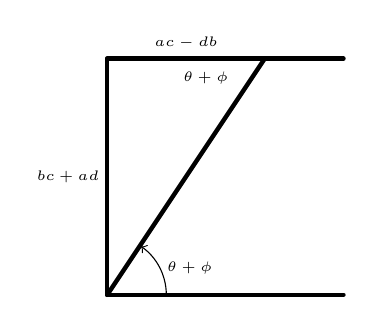
\begin{tikzpicture}[line cap=round]

  \draw [ultra thick] (0,0) -- (0,3);
  \draw [ultra thick] (0,0) -- (3,0);
  \draw [ultra thick] (0,3) -- (3,3);



  
  \draw [ultra thick] (0,0) -- (2,3);

 





  \draw [->] (.75,0) arc(0:55:.75); 
  \draw [rotate=18] (1.1,0) node {\tiny{$\theta + \phi$}};
  \draw (1.25,2.75) node {\tiny{$\theta + \phi$}};




  \draw (-0.5,1.5) node {\tiny{$bc+ad$}};
  \draw (1,3.2) node {\tiny{$ac-db$}};






    \end{tikzpicture}
  \end{image}





It is upsidedown, but this is the right triangle defined on the unit circle by adding our angles $\theta$ and $\phi$.




Let's flip it over and take a closer look.










\begin{image}[3in]
    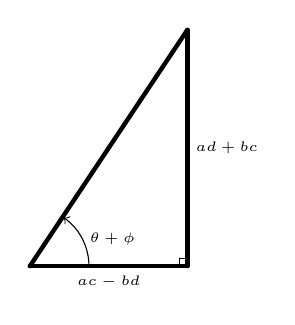
\begin{tikzpicture}[line cap=round]

  \draw [ultra thick] (0,0) -- (2,3);
  \draw [ultra thick] (0,0) -- (2,0);
  \draw [ultra thick] (2,0) -- (2,3);


  \draw [thin] (1.9,0) -- (1.9,0.1);
  \draw [thin] (1.9,0.1) -- (2,0.1);


  \draw [->] (.75,0) arc(0:55:.75); 
  \draw [rotate=18] (1.1,0) node {\tiny{$\theta + \phi$}};





  \draw (2.5,1.5) node {\tiny{$ad+bc$}};
  \draw (1,-0.2) node {\tiny{$ac-bd$}};






    \end{tikzpicture}
  \end{image}



The hypotenuse has length $1$, so it reaches out to the unit circle.

The angle is $\theta + \phi$.


What are the lengths of the sides?




 

\textcolor{red!80!black}{$\blacktriangleright$} $\cos(\theta + \phi)$ is the length of the adjacent side, which is 


\[  a \cdot c - b \cdot d = \cos(\theta) \cdot \cos(\phi) - \sin(\theta) \cdot \sin(\phi)  \]


\[  \cos(\theta + \phi) = \cos(\theta) \cdot \cos(\phi) - \sin(\theta) \cdot \sin(\phi)  \]







 

\textcolor{red!80!black}{$\blacktriangleright$} $\sin(\theta + \phi)$ is the length of the opposite side, which is 


\[  a \cdot d + b \cdot c = \cos(\theta) \cdot \sin(\phi) - \sin(\theta) \cdot \cos(\phi)  \]


\[  \sin(\theta + \phi) = \cos(\theta) \cdot \sin(\phi) - \sin(\theta) \cdot \cos(\phi)  \]














\begin{theorem}  \textbf{\textcolor{-red!75!green}{Sine and Cosine of a Sum}}

\[  \sin(\theta + \phi) = \cos(\theta) \cdot \sin(\phi) - \sin(\theta) \cdot \cos(\phi)  \]

\[  \cos(\theta + \phi) = \cos(\theta) \cdot \cos(\phi) - \sin(\theta) \cdot \sin(\phi)  \]

\end{theorem}




The difference between two angles would be adding the opposite, which means to rotate clockwise.

We have some relations to help us investigate this combination.



\begin{itemize}
\item $\sin(-\theta) = -\sin(\theta)$
\item $\cos(-\theta) = \cos(\theta)$
\end{itemize}


Now we can just think of adding again.





\begin{theorem}  \textbf{\textcolor{-red!75!green}{Sine and Cosine of a Difference}}

\[  \sin(\theta + \phi) = \cos(\theta) \cdot \sin(\phi) - \sin(\theta) \cdot \cos(\phi)  \]

\[  \cos(\theta + \phi) = \cos(\theta) \cdot \cos(\phi) - \sin(\theta) \cdot \sin(\phi)  \]

\end{theorem}













\begin{example}  Quarter Circles 


Rotating a quarter circle moves an angle into the next quadrant.  The lengths of the legs of the right triangles switch legs and the signs for sine and cosine need adjusting.



\[  \sin\left( \theta + \frac{\pi}{2} \right) = \cos(\theta) \cdot \sin\left( \frac{\pi}{2} \right) - \sin(\theta) \cdot \cos\left( \frac{\pi}{2} \right)  \]



\[  \sin\left( \theta + \frac{\pi}{2} \right) = \cos(\theta) \cdot 1 - \sin(\theta) \cdot 0  \]

\[  \sin\left( \theta + \frac{\pi}{2} \right) = \cos(\theta)  \]



\[  \cos\left( \theta + \frac{\pi}{2} \right) = \cos(\theta) \cdot \cos\left( \frac{\pi}{2} \right) - \sin(\theta) \cdot \sin\left( \frac{\pi}{2} \right)  \]

\[  \cos\left( \theta + \frac{\pi}{2} \right) = \cos(\theta) \cdot 0 - \sin(\theta) \cdot 1  \]

\[  \cos\left( \theta + \frac{\pi}{2} \right) =  - \sin(\theta)   \]




\end{example}














\begin{center}
\textbf{\textcolor{green!50!black}{ooooo-=-=-=-ooOoo-=-=-=-ooooo}} \\

more examples can be found by following this link\\ \link[More Examples of The Unit Circle]{https://ximera.osu.edu/csccmathematics/precalculus2/precalculus2/theUnitCircle/examples/exampleList}

\end{center}







\end{document}
